\chapter{自旋几何与第一个纠缠态}

\lectureoverview{纠缠属于具有部分的系统，但在单自旋的机制尚未完备之前，无法诚实地解读双自旋问题。因此，我们从沿任意轴的自旋开始，推导两个方向之间的跃迁概率，将测量解释为滤波器，并确认对易性是可观测量相容的判据。随后一个计数论证表明，两个自旋所拥有的纯态比两个分别制备的自旋所能提供的更多。多出的态是纠缠的，而最简单的例子已经具有确定的成对关联，同时每个电子单独来看则完全未极化。}

\section{完成单自旋问题}

贝尔定理可以暂且搁置。纠缠本身始于两个电子，但单电子的剩余结构将进入每一个计算。因此，在将两态系统组合成两份之前，让我们先完成它。

选择一个普通空间单位矢量
\begin{equation}
  \hat n=(n_1,n_2,n_3),
  \qquad
  n_1^2+n_2^2+n_3^2=1.
  \label{eq:l04-unit-pointer}
\end{equation}
标签\(1,2,3\)同样可以称为\(x,y,z\)。重要的是这些轴构成一个一致的右手坐标系。

\begin{classroomqa}
\lecturetimestamp{00:02:33}
\audiencequestion{黑板上画的坐标三轴是右手的吗？}
\lecturerresponse{第一幅草图是左手的。反转第二个轴，或一致地重新标记两个轴，即可修正。下面的计算只使用固定的右手约定；草图的偶然取向不携带任何物理。}
\end{classroomqa}

自旋有三个可观测分量，由泡利矩阵表示
\begin{equation}
  \begin{aligned}
    \sigma_1&=
    \begin{pmatrix}0&1\\1&0\end{pmatrix},
    &
    \sigma_2&=
    \begin{pmatrix}0&-i\\i&0\end{pmatrix},\\[0.5em]
    \sigma_3&=
    \begin{pmatrix}1&0\\0&-1\end{pmatrix}.
  \end{aligned}
\end{equation}
沿\(\hat n\)的分量是指针与该矩阵值矢量的普通空间点积：
\begin{equation}
  \sigma_{\hat n}
  \equiv
  \boldsymbol{\sigma}\cdot\hat n
  =
  n_1\sigma_1+n_2\sigma_2+n_3\sigma_3.
  \label{eq:l04-sigma-dot-n}
\end{equation}
这个点积是在物理三维空间中进行的。它不是两个态矢量的内积。

\begin{figure}[htbp]
\centering
\includegraphics[width=0.82\linewidth]{lecture_04_figure_02.png}
\caption{沿\(\hat n\)的空间分量成为三个矩阵可观测量的线性组合。}
\lectureframe{00:05:09}
\end{figure}

代入泡利矩阵得到
\begin{equation}
  \sigma_{\hat n}
  =
  \begin{pmatrix}
    n_3 & n_1-in_2\\
    n_1+in_2 & -n_3
  \end{pmatrix}.
  \label{eq:l04-sigma-n-matrix}
\end{equation}
方便起见缩写为
\begin{equation}
  n_-=n_1-in_2,
  \qquad
  n_+=n_1+in_2=n_-^*,
\end{equation}
于是
\begin{equation}
  \sigma_{\hat n}
  =
  \begin{pmatrix}
    n_3&n_-\\
    n_+&-n_3
  \end{pmatrix}.
\end{equation}
实对角元和共轭非对角元使该算符为厄米的。

\begin{figure}[htbp]
\centering
\includegraphics[width=0.84\linewidth]{lecture_04_figure_03.png}
\caption{任意轴自旋可观测量的显式二乘二形式。}
\lectureframe{00:07:34}
\end{figure}

在操作上，测量\(\sigma_{\hat n}\)意味着将强磁场沿\(\hat n\)取向，并观察自旋相关的响应，在讲座中以是否发射光子来表示。矩阵与实验室中的问题是对同一次测量的两种描述。

两个小恒等式将支撑余下的计算。首先，
\begin{equation}
  \sigma_{\hat n}^{\,2}=I.
  \label{eq:l04-sigma-n-square}
\end{equation}
这可以通过将方程~\eqref{eq:l04-sigma-n-matrix}自乘，或利用
\begin{equation}
  \sigma_i^2=I,
  \qquad
  \sigma_i\sigma_j=-\sigma_j\sigma_i
  \quad(i\ne j).
\end{equation}
来得到。因此\(\sigma_{\hat n}\)的每个本征值\(\lambda\)都满足\(\lambda^2=1\)，所以唯一可能的结果是
\begin{equation}
  \lambda=\pm1.
\end{equation}
其次，
\begin{equation}
  n_+n_-
  =n_1^2+n_2^2
  =1-n_3^2
  =(1-n_3)(1+n_3).
  \label{eq:l04-nplus-nminus}
\end{equation}
这不是什么深刻的定理，但正是这个恒等式使本征矢代数保持可控。

\section{从制备到概率}

将电子制备为沿\(\hat n\)的自旋\(+1\)，然后沿另一个方向\(\hat m\)测量。核心的单自旋问题是
\begin{equation}
  P(m,+\mid n,+)
  =
  P(\sigma_{\hat m}=+1\mid\sigma_{\hat n}=+1).
  \label{eq:l04-central-probability}
\end{equation}
对称性提示答案应只依赖于\(\hat n\)与\(\hat m\)之间的夹角，并且交换这两个方向不应改变它。这些预期是有用的检验，但不能替代概率公设。

\begin{classroomqa}
\lecturetimestamp{00:14:03}
\audiencequestion{量子力学本身是否告诉我们三个泡利矩阵就是自旋算符，还是这是从实验中学到的？}
\lecturerresponse{这一认定是量子力学累积经验结构的一部分，而不是某个孤立实验的结果。反复的自旋实验揭示了概率规律，而矩阵形式体系是经由爱因斯坦、玻恩、海森堡、狄拉克等人的工作建立起来以编码这些规律的。这些公设是受数据约束的、极为成功的猜测。}
\end{classroomqa}

令
\begin{equation}
  \sigma_{\hat n}\ket{n,+}=\ket{n,+},
  \qquad
  \sigma_{\hat m}\ket{m,+}=\ket{m,+}.
  \label{eq:l04-nm-eigenstates}
\end{equation}
符号\(n,+\)和\(m,+\)是右矢内部的标签。它们标识本征值为\(+1\)的本征态。

\begin{figure}[htbp]
\centering
\includegraphics[width=0.76\linewidth]{lecture_04_figure_04.png}
\caption{沿\(\hat n\)和\(\hat m\)的自旋的\(+1\)本征态。}
\lectureframe{00:17:36}
\end{figure}

首先要计算的量是概率幅
\begin{equation}
  \mathcal A(m,+\mid n,+)=\braket{m,+}{n,+}.
\end{equation}
概率是其绝对值的平方：
\begin{equation}
  P(m,+\mid n,+)
  =
  \left|\braket{m,+}{n,+}\right|^2.
  \label{eq:l04-born-nm}
\end{equation}
先振幅，后概率：这个顺序是本质性的量子步骤。

\begin{figure}[htbp]
\centering
\includegraphics[width=0.78\linewidth]{lecture_04_figure_05.png}
\caption{制备的\(n\)态与所检验的\(m\)态之间的重叠就是概率幅。}
\lectureframe{00:19:59}
\end{figure}

\subsection{求解本征态}

将\(\sigma_{\hat n}\)的一个候选\(+1\)本征向量写为
\begin{equation}
  \begin{pmatrix}\alpha\\\beta\end{pmatrix}.
\end{equation}
归一化可以稍后再处理，而整体相位没有物理效应。因此，在南极点坐标片之外，我们可以取\(\alpha=1\)并写出\(\beta=z\)。
\begin{equation}
  \begin{pmatrix}
    n_3&n_-\\
    n_+&-n_3
  \end{pmatrix}
  \begin{pmatrix}1\\z\end{pmatrix}
  =
  \begin{pmatrix}1\\z\end{pmatrix}
\end{equation}
的上分量给出
\begin{equation}
  n_3+n_-z=1,
  \qquad
  z=\frac{1-n_3}{n_-}.
  \label{eq:l04-z-solution}
\end{equation}
一旦使用方程~\eqref{eq:l04-nplus-nminus}，下分量给出相同的条件。

该未归一化向量的模方为
\begin{align}
  \begin{pmatrix}
    1&\dfrac{1-n_3}{n_+}
  \end{pmatrix}
  \begin{pmatrix}
    1\\[3pt]\dfrac{1-n_3}{n_-}
  \end{pmatrix}
  &=
  1+\frac{(1-n_3)^2}{n_+n_-}
  \notag\\
  &=
  1+\frac{1-n_3}{1+n_3}
  =
  \frac{2}{1+n_3}.
  \label{eq:l04-unnormalized-norm}
\end{align}
因此，一个归一化的选择是
\begin{equation}
  \ket{n,+}
  =
  \sqrt{\frac{1+n_3}{2}}
  \begin{pmatrix}
    1\\[5pt]\dfrac{1-n_3}{n_-}
  \end{pmatrix}.
  \label{eq:l04-normalized-n-state}
\end{equation}
在\(n_3=-1\)处，这个坐标表达式是奇异的，尽管态本身并非如此；本征态就是\(\ket d=(0,1)^T\)。奇异性属于相位约定，而不属于自旋。

将\(n\)替换为\(m\)并取复共轭，得到
\begin{equation}
  \bra{m,+}
  =
  \sqrt{\frac{1+m_3}{2}}
  \begin{pmatrix}
    1&
    \dfrac{1-m_3}{m_+}
  \end{pmatrix}.
\end{equation}
这个内积看起来并不好看，而将其乘以自身的复共轭看起来更糟。反复使用方程~\eqref{eq:l04-nplus-nminus}可将结果化简为
\begin{equation}
  \begin{aligned}
    P(m,+\mid n,+)
    &=\frac{1+n_1m_1+n_2m_2+n_3m_3}{2}\\
    &=\frac{1+\hat n\cdot\hat m}{2}.
  \end{aligned}
  \label{eq:l04-spin-transition-probability}
\end{equation}
若\(\theta_{nm}\)是两个空间方向之间的夹角，则
\begin{equation}
  P(m,+\mid n,+)
  =
  \frac{1+\cos\theta_{nm}}{2}
  =
  \cos^2\frac{\theta_{nm}}{2}.
  \label{eq:l04-half-angle-probability}
\end{equation}

\begin{classroomqa}
\lecturetimestamp{00:32:47}
\audiencequestion{两个态正交，是否意味着内积必须为零？}
\lecturerresponse{不。标记\(m,+\)和\(n,+\)指的是不同的测量轴，而不是同一个固定可观测量的不同本征值。若\(m=n\)，则两个态重合，其内积为一。只有当物理方向相反时，它们才正交，从而一个态是同一自旋分量的\(+1\)态，另一个是\(-1\)态。}
\end{classroomqa}

\section{概率公式意味着什么}

方程~\eqref{eq:l04-spin-transition-probability}立即通过三项检验：
\begin{align}
  \hat m=\hat n
  &\quad\Longrightarrow\quad P=1,
  \notag\\
  \hat m=-\hat n
  &\quad\Longrightarrow\quad P=0,
  \notag\\
  \hat m\cdot\hat n=0
  &\quad\Longrightarrow\quad P=\frac12.
\end{align}
答案只依赖于相对角度，并且在\(m\leftrightarrow n\)下对称。旋转整个装置不会改变任何预言。

这就是自旋二分之一所作出的非凡妥协。沿每一条轴，观测结果仍然是\(+1\)或\(-1\)，从来不是分数自旋值。光滑的旋转依赖性反而出现在这两个离散答案的概率中。

\begin{classroomqa}
\lecturetimestamp{00:39:20}
\audiencequestion{我们怎么知道重复试验涉及的是同一个电子，概率又是如何测量的？}
\lecturerresponse{可以把一个电子限制在腔内，并通过其电通量监测守恒电荷，将该电子沿\(\hat n\)重新制备，然后沿\(\hat m\)重复测量。等价地，也可以制备大量全同电子，并对每个电子测量一次。在统计误差范围内，两种做法中正、负结果的长期比率相同。}
\end{classroomqa}

\begin{classroomqa}
\lecturetimestamp{00:41:29}
\audiencequestion{系综中的所有成员都必须在一个集体实验中测量吗？}
\lecturerresponse{不。每个成员都按相同方案制备，并分别测量。一百万次这样的试验构成一个统计实验，仅仅是在其结果频率估计同一概率的意义上。}
\end{classroomqa}

\begin{classroomqa}
\lecturetimestamp{00:42:23}
\audiencequestion{如果一个电子被重复使用，它能发射多少个光子？}
\lecturerresponse{不存在固定的寿命配额。每个循环在磁场开启时都包含外部做功。如果自旋处于较高能量的取向，那么所供给的能量可以在弛豫过程中以光子形式离开。因此，原则上该装置可以无限重复制备—发射循环。}
\end{classroomqa}

在已知旋转不变性之后，这个公式可以非常快地得到：选择\(\hat n\)作为第三轴，于是\(\ket{n,+}=(1,0)^T\)，并从\(\ket{m,+}\)的上分量读出概率。但一开始就使用这个捷径，会预设显式计算刚刚证明的对称性。

\begin{classroomqa}
\lecturetimestamp{00:43:33}
\audiencequestion{更好的基选择能否消除难看的任意轴本征向量？}
\lecturerresponse{能。一旦有了旋转和幺正变换，就可以让一条坐标轴与其中一个方向对齐，从而使计算变短。在这个阶段，显式计算有其目的：它验证所选的泡利矩阵确实给出旋转不变的答案，而不是预设这一事实。}
\end{classroomqa}

\begin{classroomqa}
\lecturetimestamp{00:48:30}
\audiencequestion{答案只依赖于角度的物理原因是什么？}
\lecturerresponse{结构性的答案属于量子对称性理论：空间旋转由作用在自旋态和可观测量上的幺正变换表示。那套语言稍后才会出现。目前，角度依赖性是泡利矩阵计算所赢得的结果。}
\end{classroomqa}

\section{测量是一个滤波器}

测量不仅仅报告一个数值。如果测量\(\sigma_{\hat m}\)，结果为\(+1\)，则电子被留在\(\ket{m,+}\)。该装置既充当探测器，又充当态制备器，正如偏振器检验光子并让透射光子沿其自身轴偏振一样。

这条态变化规则使同时测量的问题变得具体。两个可观测量只有在存在同时是二者本征矢量的态时，才能一起具有可重复的确定值。

\begin{classroomqa}
\lecturetimestamp{00:51:29}
\audiencequestion{一次测量能否同时确定两个不同的自旋分量，例如\(\sigma_1\)和\(\sigma_2\)？}
\lecturerresponse{不能。它们的本征矢量不同。测量其中一个分量会把电子留在该分量的一个本征态中，但该态不是另一个分量的本征态。因此，第一次测量破坏了第二次测量所要求的确定性。}
\end{classroomqa}

一般有限维的陈述对厄米算符表述得最为简洁。

\begin{theorem}
两个厄米算符\(A\)和\(B\)可同时对角化，当且仅当它们对易：
\begin{equation}
  [A,B]\equiv AB-BA=0.
  \label{eq:l04-commutator}
\end{equation}
等价地说，它们允许一个完备的共同正交归一本征基。\end{theorem}

对于容易的方向，假设
\begin{equation}
  A\ket{\alpha_i}=\lambda_i\ket{\alpha_i},
  \qquad
  B\ket{\alpha_i}=\mu_i\ket{\alpha_i}
\end{equation}
对某个完备基成立。那么
\begin{align}
  AB\ket{\alpha_i}
  &=\lambda_i\mu_i\ket{\alpha_i},
  \notag\\
  BA\ket{\alpha_i}
  &=\mu_i\lambda_i\ket{\alpha_i},
\end{align}
所以\(AB\)和\(BA\)在每个基矢量上一致。因此\(AB=BA\)。反过来，如果厄米算符\(A\)和\(B\)对易，则\(B\)保持\(A\)的每个本征空间不变；在任意简并本征空间内将\(B\)对角化，就产生一个共同本征基。

\begin{figure}[htbp]
\centering
\includegraphics[width=0.76\linewidth]{lecture_04_figure_06.png}
\caption{两个可观测量可以具有相同的本征矢量，却给它们赋予不同的本征值。}
\lectureframe{00:55:45}
\end{figure}

\begin{classroomqa}
\lecturetimestamp{00:53:56}
\audiencequestion{我们能否同时沿\(x\)和\(y\)施加磁场，并称之为同时测量？}
\lecturerresponse{这些场相加为一个合方向。于是该装置测量沿那个合轴的自旋，也许是在\(45^\circ\)处，而不是分别测量\(\sigma_x\)和\(\sigma_y\)。所尝试的构造产生的是第三个可观测量，而不是两个相容的读数。}
\end{classroomqa}

\section{每个纯单自旋态都有一个轴}

现在反转本征矢量问题。给定一个任意归一化旋量
\begin{equation}
  \ket\psi=
  \begin{pmatrix}\alpha\\\beta\end{pmatrix},
  \qquad
  |\alpha|^2+|\beta|^2=1,
  \label{eq:l04-general-spinor}
\end{equation}
是否存在某个空间方向\(\hat n\)满足
\begin{equation}
  \sigma_{\hat n}\ket\psi=\ket\psi?
  \label{eq:l04-reverse-eigenproblem}
\end{equation}
存在。讲座首先通过计数看出原因。两个复分量包含四个实数。归一化去掉一个，物理上无关的整体相位再去掉一个，剩下两个。单位指针也有两个独立的实参数，例如经度和纬度。

\begin{classroomqa}
\lecturetimestamp{01:03:52}
\audiencequestion{既然\(\alpha\)和\(\beta\)都是复数，这个态怎么只有两个自由度？}
\lecturerresponse{它们从四个实分量开始。归一化条件去掉一个实自由度，而将整个态乘以\(e^{i\theta}\)不改变任何概率，所以共同相位又去掉一个。剩下两个物理上有意义的参数，与单位指针的两个角相匹配。}
\end{classroomqa}

\begin{classroomqa}
\lecturetimestamp{01:04:20}
\audiencequestion{我们还需要解出本征值吗？}
\lecturerresponse{这里目标本征值固定为\(+1\)。我们只寻找其自旋向上态为给定旋量的方向。相反的指针会把同一条射线描述为本征值为\(-1\)的自旋向下态。}
\end{classroomqa}

计数解释了为什么这种对应关系应当存在。直接构造证实了它。定义
\begin{align}
  n_1&=\bra\psi\sigma_1\ket\psi
      =2\operatorname{Re}(\alpha^*\beta),
  \notag\\
  n_2&=\bra\psi\sigma_2\ket\psi
      =2\operatorname{Im}(\alpha^*\beta),
  \notag\\
  n_3&=\bra\psi\sigma_3\ket\psi
      =|\alpha|^2-|\beta|^2.
  \label{eq:l04-bloch-components}
\end{align}
归一化给出\(n_1^2+n_2^2+n_3^2=1\)，直接代入给出式~\eqref{eq:l04-reverse-eigenproblem}。因此，每个纯单自旋态都沿某个空间轴自旋向上。

这个陈述有一个操作版本。制备同一个未知纯态的许多副本。沿试探方向分批测量，调整磁体，并寻找使每个结果都为自旋向上的方向。有限数据只能在不确定度范围内确定该方向，但理想态有一个精确的轴。

提问是这种方法的一部分，而不是对它的打断。一段简短的课堂插叙回忆起十岁孩子自由地询问弦理论、额外维度，以及周围的中微子是否会引起头痛。问题的细节可能是错的；暴露困惑之处的意愿仍然宝贵。

\section{两个自旋与局域算符}

在组合两个自旋之前，记录泡利矩阵如何作用于\(\sigma_3\)基：
\begin{align}
  \sigma_1\ket u&=\ket d,
  &
  \sigma_1\ket d&=\ket u,
  \notag\\
  \sigma_2\ket u&=i\ket d,
  &
  \sigma_2\ket d&=-i\ket u,
  \notag\\
  \sigma_3\ket u&=\ket u,
  &
  \sigma_3\ket d&=-\ket d.
  \label{eq:l04-pauli-action-table}
\end{align}

\begin{figure}[htbp]
\centering
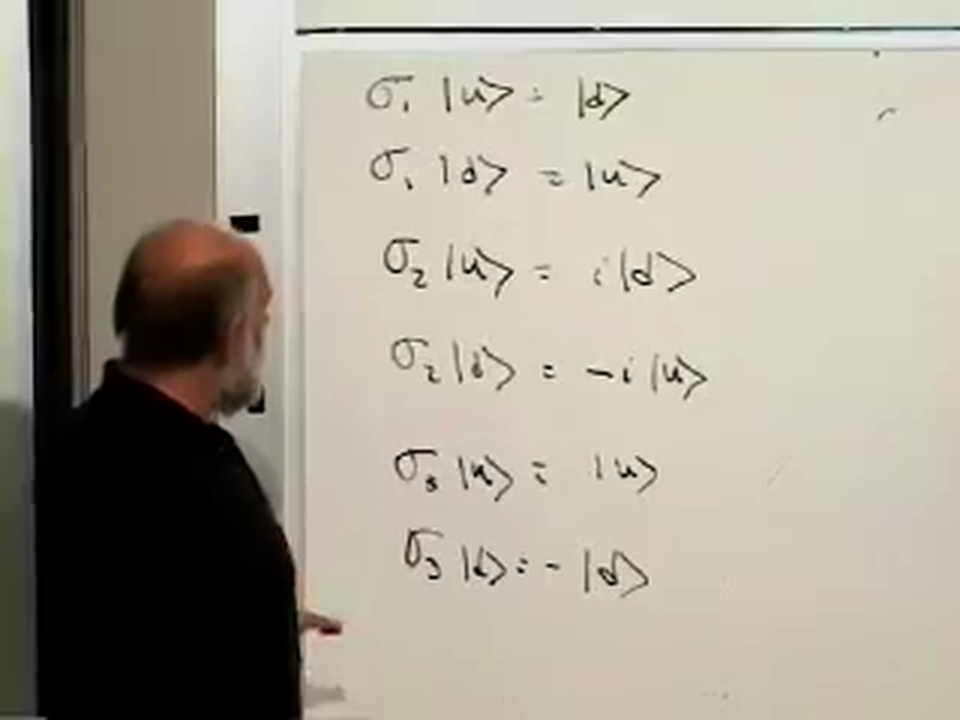
\includegraphics[width=0.80\linewidth]{lecture_04_figure_07.png}
\caption{泡利作用表把矩阵重新表述为作用于自旋向上/向下基的规则。}
\lectureframe{01:09:35}
\end{figure}

现在设想两个电子被置于可区分的位置，因此只有它们的自旋会变化。四个基态是
\begin{equation}
  \ket{uu},
  \qquad
  \ket{du},
  \qquad
  \ket{ud},
  \qquad
  \ket{dd}.
  \label{eq:l04-two-spin-basis}
\end{equation}
第一个标签属于电子\(1\)，第二个属于电子\(2\)。它们相互正交归一，因为它们表示两个第三分量测量的不同联合结果。

\begin{figure}[htbp]
\centering
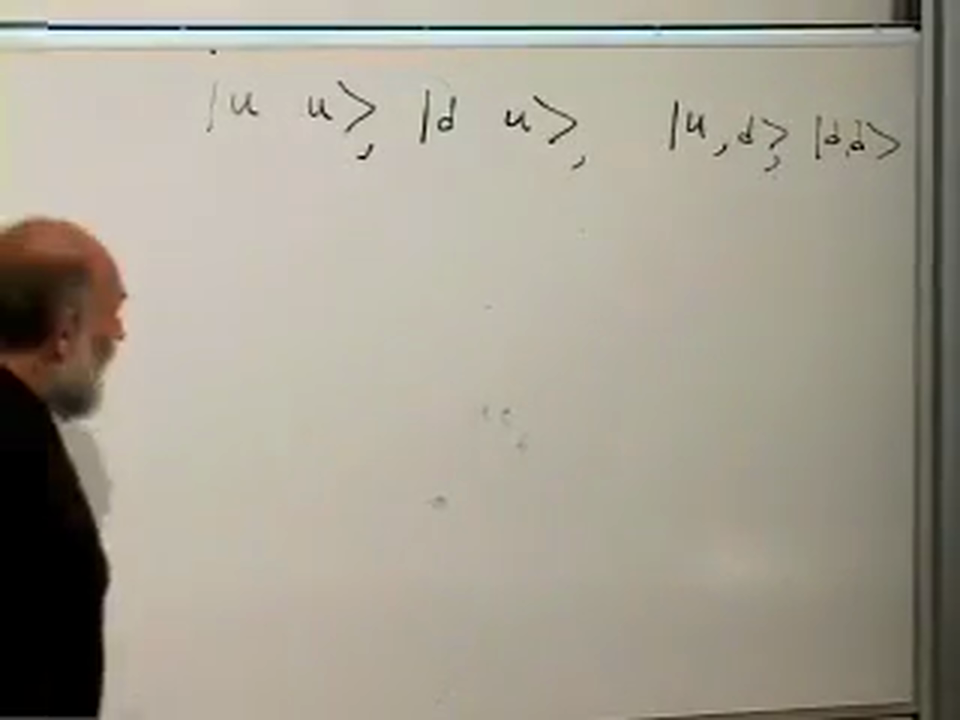
\includegraphics[width=0.82\linewidth]{lecture_04_figure_08.png}
\caption{这四个乘积基标签张成双自旋态空间。}
\lectureframe{01:11:40}
\end{figure}

把作用于电子\(1\)的算符记作\(\sigma_i\)，把作用于电子\(2\)的算符记作\(\tau_i\)。更明确地说，
\begin{equation}
  \sigma_i\equiv\sigma_i\otimes I,
  \qquad
  \tau_i\equiv I\otimes\sigma_i.
\end{equation}
第一组只作用于第一个标签，而第二组只作用于第二个：
\begin{align}
  \sigma_1\ket{ud}&=\ket{dd},
  &
  \sigma_1\ket{dd}&=\ket{ud},
  \notag\\
  \sigma_3\ket{dd}&=-\ket{dd},
  &
  \tau_2\ket{ud}&=-i\ket{uu}.
  \label{eq:l04-local-operator-examples}
\end{align}
一旦一个算符对四个基态的作用已知，线性性就决定了它对每个双自旋态的作用。

\begin{classroomqa}
\lecturetimestamp{01:17:47}
\audiencequestion{为什么因子\(-i\)写在右矢外面？它作用于两个电子吗？}
\lecturerresponse{右矢内部的符号是基组态的标签。一个复标量乘的是整个态矢量，所以标准记号把它放在外面。它在这里的来源是\(\tau_2\)对第二个标签的作用；把它写在外面并不意味着对两个电子施加了一个单独的物理操作。}
\end{classroomqa}

\begin{classroomqa}
\lecturetimestamp{01:19:44}
\audiencequestion{乘以\(i\)是否表示电子在普通空间中的旋转？}
\lecturerresponse{单凭它本身并不表示。它是态空间中的复标量乘法。空间旋转稍后将由特定的酉算符表示；在这个作用表中一个孤立的因子\(i\)并不是字面意义上的实空间转动。}
\end{classroomqa}

\section{六个参数，而非四个}

这对粒子的一般纯态是
\begin{equation}
  \ket\Psi
  =
  c_{uu}\ket{uu}
  +c_{du}\ket{du}
  +c_{ud}\ket{ud}
  +c_{dd}\ket{dd}.
  \label{eq:l04-general-two-spin-state}
\end{equation}
四个复系数给出八个实数。归一化去掉一个，整体相位去掉一个：
\begin{equation}
  8-1-1=6.
  \label{eq:l04-two-spin-parameter-count}
\end{equation}
单独制备的电子\(1\)纯态需要两个实参数，电子\(2\)还需要两个，总共只有四个。缺失的两个参数不是记账错误。它们标志着这对粒子的某些纯态不能为各部分分别指定纯态。

首先找出确实来自分别制备的态。如果
\begin{equation}
  \ket{\psi_1}=\alpha_1\ket u+\beta_1\ket d,
  \qquad
  \ket{\psi_2}=\alpha_2\ket u+\beta_2\ket d,
\end{equation}
那么
\begin{align}
  \ket{\psi_1}\otimes\ket{\psi_2}
  &=
  \alpha_1\alpha_2\ket{uu}
  +\alpha_1\beta_2\ket{ud}
  \notag\\
  &\quad
  +\beta_1\alpha_2\ket{du}
  +\beta_1\beta_2\ket{dd}.
  \label{eq:l04-product-expansion}
\end{align}
这是一个\emph{乘积态}。每个电子都有自己的极化轴，正如两次磁制备独立进行时那样。

\begin{figure}[htbp]
\centering
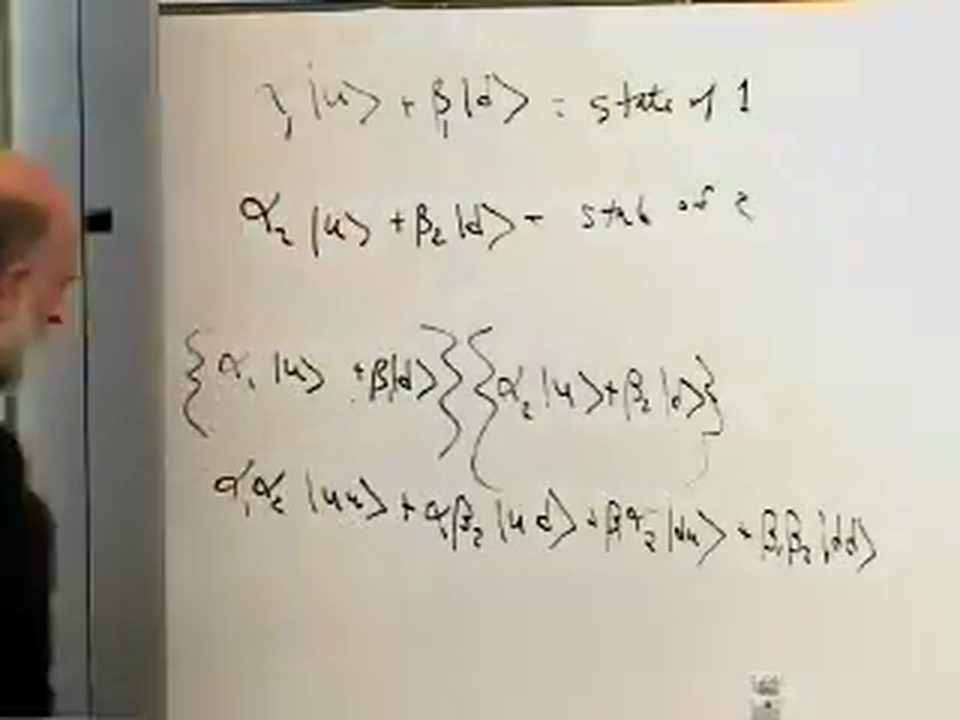
\includegraphics[width=0.84\linewidth]{lecture_04_figure_09.png}
\caption{两个单自旋态相乘产生一个受限的四项乘积态。}
\lectureframe{01:25:15}
\end{figure}

如果四个系数排列为
\begin{equation}
  C=
  \begin{pmatrix}
    c_{uu}&c_{ud}\\
    c_{du}&c_{dd}
  \end{pmatrix},
\end{equation}
那么该态是乘积态，当且仅当\(C\)的秩为一，等价地
\begin{equation}
  c_{uu}c_{dd}-c_{ud}c_{du}=0.
  \label{eq:l04-product-condition}
\end{equation}
大多数四个振幅的选择不满足这个条件。它们是纠缠的。

\section{第一个纠缠态}

讲座的第一个例子是
\begin{equation}
  \ket{\psi_+}
  =
  \frac{1}{\sqrt2}
  \left(\ket{ud}+\ket{du}\right).
  \label{eq:l04-psi-plus}
\end{equation}
它不能分解为电子\(1\)的一个态和电子\(2\)的一个态。如果第三轴测量发现电子\(2\)向下，那么电子\(1\)向上；如果发现电子\(2\)向上，那么电子\(1\)向下。这对粒子具有确定的、两个粒子各自都不拥有的信息。

\begin{figure}[htbp]
\centering
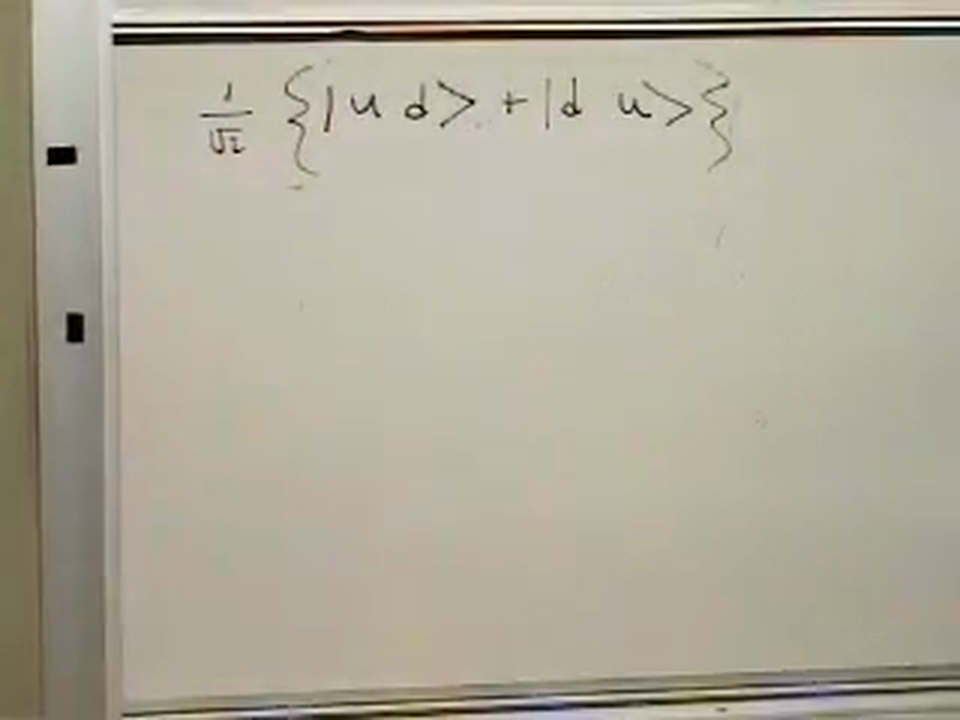
\includegraphics[width=0.82\linewidth]{lecture_04_figure_10.png}
\caption{第一个纠缠叠加包含一个向上和一个向下，但并未事先把任一结果分配给某个粒子。}
\lectureframe{01:29:30}
\end{figure}

要看出任一电子单独看起来是什么样，计算三个局域期望值。对于第一分量，
\begin{equation}
  \sigma_1\ket{\psi_+}
  =
  \frac{1}{\sqrt2}
  \left(\ket{dd}+\ket{uu}\right),
\end{equation}
它与\(\ket{\psi_+}\)正交。因此
\begin{equation}
  \bra{\psi_+}\sigma_1\ket{\psi_+}=0.
\end{equation}
类似地，
\begin{equation}
  \sigma_2\ket{\psi_+}
  =
  \frac{i}{\sqrt2}
  \left(\ket{dd}-\ket{uu}\right),
\end{equation}
所以
\begin{equation}
  \bra{\psi_+}\sigma_2\ket{\psi_+}=0.
\end{equation}
对于第三分量，
\begin{equation}
  \sigma_3\ket{\psi_+}
  =
  \frac{1}{\sqrt2}
  \left(\ket{ud}-\ket{du}\right),
\end{equation}
两个对角贡献相消：
\begin{equation}
  \bra{\psi_+}\sigma_3\ket{\psi_+}
  =\frac12(1-1)=0.
\end{equation}
因此
\begin{equation}
  \begin{aligned}
    \bra{\psi_+}\sigma_i\ket{\psi_+}&=0,\\
    \bra{\psi_+}\tau_i\ket{\psi_+}&=0,
    \qquad i=1,2,3.
  \end{aligned}
  \label{eq:l04-zero-local-spin}
\end{equation}

\begin{figure}[htbp]
\centering
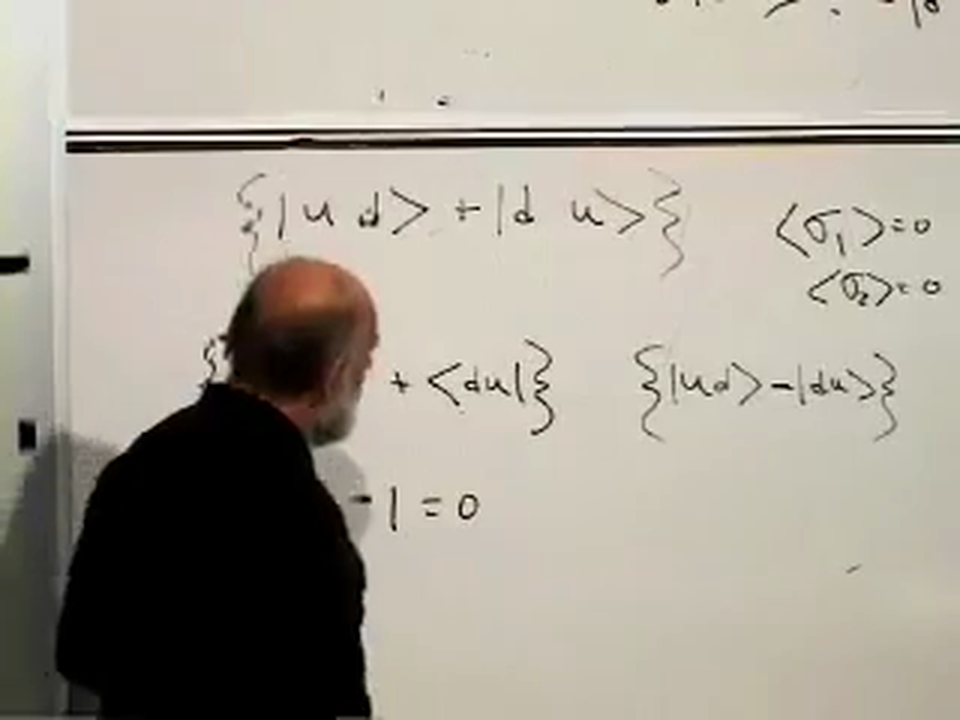
\includegraphics[width=0.84\linewidth]{lecture_04_figure_11.png}
\caption{变换后的态与相消\(1-1=0\)确立了局域自旋期望值为零。}
\lectureframe{01:35:50}
\end{figure}

对于任意方向，
\begin{equation}
  \bra{\psi_+}\sigma_{\hat n}\ket{\psi_+}=0,
  \qquad
  \bra{\psi_+}\tau_{\hat n}\ket{\psi_+}=0.
  \label{eq:l04-zero-arbitrary-local-spin}
\end{equation}
由于每个局域测量只有结果\(\pm1\)，期望值为零意味着
\begin{equation}
  P(\sigma_{\hat n}=+1)
  =
  P(\sigma_{\hat n}=-1)
  =
  \frac12,
\end{equation}
第二个电子也同样。没有任何方向能使任一电子单独极化。这对单自旋纯态是不可能的，但对纠缠纯态的一部分却完全可能。

\begin{classroomqa}
\lecturetimestamp{01:38:23}
\audiencequestion{局域结果各占一半，以及测量一个电子能让我们获知另一个电子的信息，这两者是同一个论断吗？}
\lecturerresponse{不是。首先忽略电子\(2\)：仅对电子\(1\)测量任意方向，都给出各占一半的分布。这确立了不存在任何局域极化。关联则是关于两个记录结果如何相互联系的独立联合陈述。纠缠同时提供这两个特征，但不应用其中一个来代替对另一个的证明。}
\end{classroomqa}

\section{贝尔之前的关联}

关联本身并不唯一地属于量子。把一枚便士和一枚角币混在一起，不看它们就把它们分开，然后检查其中一枚。检查之前，任一物体是便士的概率都是五五开，但在这里发现便士就告诉我们远处的物体是角币。即使任一部分单独并不携带确定信息，这一对物体仍携带确定信息。

\begin{classroomqa}
\lecturetimestamp{01:41:45}
\audiencequestion{便士—角币的推断是否只有在我们知道原来那一对中恰好各有一枚时才成立？}
\lecturerresponse{正是如此。经典推断依赖于可信的制备。同样，量子关联预言只有在双电子系统已被制备到指定的联合态时才适用。}
\end{classroomqa}

\begin{classroomqa}
\lecturetimestamp{01:42:09}
\audiencequestion{对于\(\ket{\psi_+}\)，两个第三分量测量都向上的概率是否等于零？这是否证明自旋沿每个轴都相反？}
\lecturerresponse{在第三轴基下，\(uu\)的概率为零，且两个第三轴结果是相反的。但第二个结论对这个正号态来说过强了。它的局域自旋在每个方向都为零，而它的联合关联依赖于方向。普遍相反的结果属于本讲末尾引入的负号单态。}
\end{classroomqa}

\begin{classroomqa}
\lecturetimestamp{01:43:51}
\audiencequestion{能否把经典的一对想象成两枚焊在一起的硬币，使一个面总是与另一个面相反？}
\lecturerresponse{对于固定的反关联，这是一种可能的经典机制，前提是摇晃不扰动这种连接。它仍然是一种在制备时确立的隐变量经典安排。这个类比是刻意暂定的；贝尔定理将检验每一种这样的经典解释在哪里失败。}
\end{classroomqa}

\begin{classroomqa}
\lecturetimestamp{01:44:32}
\audiencequestion{如果一个结果已经决定了伙伴的结果，大数定律又在哪里起作用？}
\lecturerresponse{条件确定性是在给定联合态和一个结果后，关于单次试验的陈述。仍然需要重复试验，以在实验上验证所承诺的关联是可靠的，并估计期望值和不完美概率。大数定律把这些重复频率与理论分布联系起来。}
\end{classroomqa}

两个观察者可能被极其巨大的距离分开。观察一个结果会改变局域观察者对另一个结果所知道的内容，但它不会向远处的观察者发送可控信息。在这个阶段，情况仍然类似于分开的便士和角币。

\begin{classroomqa}
\lecturetimestamp{01:46:46}
\audiencequestion{分开的便士—角币图景是思考量子对的正确方式吗？}
\lecturerresponse{它是正确的第一个经典比较，而不是最终的量子解释。贝尔定理关注的是携带预先存在的经典属性的一对与纠缠量子对之间可测量的差异。这一区分被推迟到必要的关联被计算出来之后。}
\end{classroomqa}

\section{单态及其制备}

在黑板计算的末尾，把加号换成减号：
\begin{equation}
  \ket{\psi_-}
  =
  \frac{1}{\sqrt2}
  \left(\ket{ud}-\ket{du}\right).
  \label{eq:l04-singlet}
\end{equation}
这一改变使方程~\eqref{eq:l04-zero-local-spin}中的局域期望值仍等于零，并使第三轴结果仍相反。它确实改变了横向联合关联。这个负号态就是自旋单态，即两个自旋沿每个共同测量轴都相反的那个旋转不变态。

\begin{figure}[htbp]
\centering
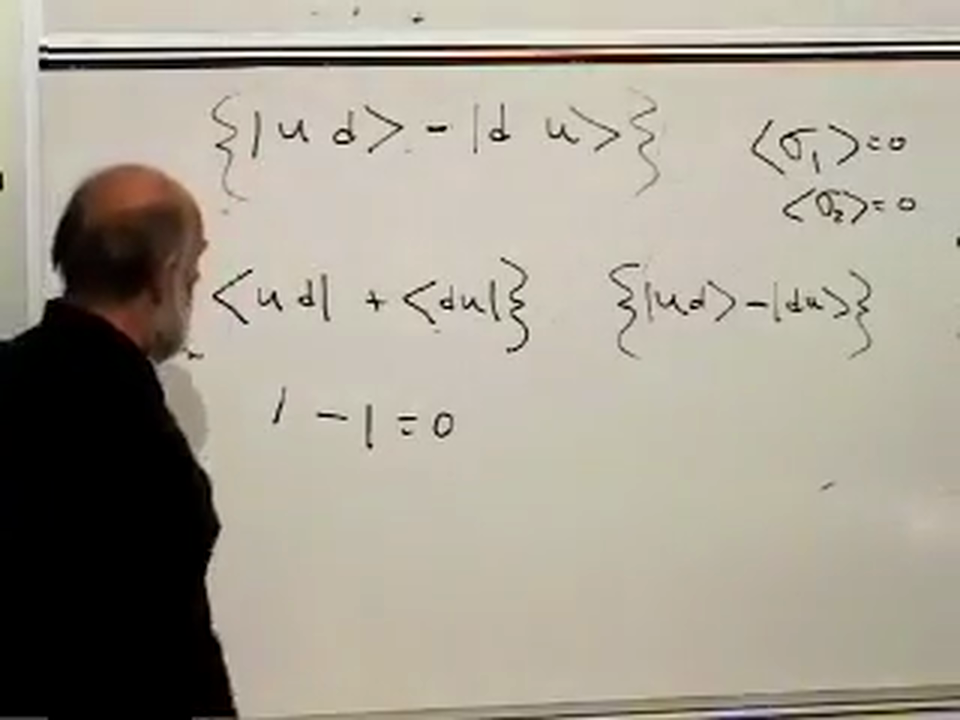
\includegraphics[width=0.84\linewidth]{lecture_04_figure_12.png}
\caption{最后的黑板改动把对称叠加替换为负号单态，同时保持局域自旋为零。}
\lectureframe{01:47:25}
\end{figure}

在这里使用的简化物理图景中，让两个局域电子磁矩靠近到足以相互作用，会使较高能量的排列通过光子发射而弛豫。在没有优先外轴的情况下，较低的自旋态由旋转对称的单态表示。确切的相互作用以及相对相位为何必须为负，需要进一步计算。

\begin{classroomqa}
\lecturetimestamp{01:49:02}
\audiencequestion{实际的制备是否仅仅是把两个电子靠近并等待？}
\lecturerresponse{在这个理想化模型中，是的：让自旋-自旋相互作用起作用，并允许辐射弛豫到较低状态。电子只需足够接近、持续足够长时间，使其磁相互作用有效即可。真实的制备方案还必须控制轨道态和竞争性相互作用。}
\end{classroomqa}

\begin{classroomqa}
\lecturetimestamp{01:49:16}
\audiencequestion{这仅仅是泡利不相容原理吗？}
\lecturerresponse{不是。这两个电子已被赋予可区分的空间位置，因此它们的自旋讨论尚不需要对重叠的轨道波函数进行反对称化。当相同的电子占据重叠的单粒子态时，不相容原理才变得相关；而目前的纠缠论证对于分离的格点已经成立。}
\end{classroomqa}

\begin{classroomqa}
\lecturetimestamp{01:50:31}
\audiencequestion{普通的电子束会自然地包含这种相互作用的电子对吗？}
\lecturerresponse{通常不会。电子束是稀薄的，典型电子在可用的飞行时间内彼此相距太远，无法产生可观的spin-spin相互作用。碰撞或刻意施加的约束相互作用可以产生纠缠电子对，但仅仅同处一束并不能。}
\end{classroomqa}

\begin{classroomqa}
\lecturetimestamp{01:51:45}
\audiencequestion{磁相互作用需要多大的距离？}
\lecturerresponse{不存在普适的明确截断；决定性的量是相互作用时间尺度。讲座给出了快速耦合的粗略微观估计，量级为\(10^{-11}\,\mathrm{cm}\)。在更大的间距下，能量分裂更小，发射的光子波长更长，弛豫所需时间要长得多。原则上足够长的等待可以补偿，而普通电子束提供的时间太少。}
\end{classroomqa}

\begin{classroomqa}
\lecturetimestamp{01:53:10}
\audiencequestion{为什么单态必须包含负号而不是正号？}
\lecturerresponse{从局部的各半统计来看这并不明显，因为对于这两个相对相位，这些统计是相同的。答案在于该态在旋转下如何变换，以及相互作用如何选择总自旋为零。推导属于下一讲。}
\end{classroomqa}

课程现在已跨过预期的门槛。单个纯自旋总是具有确定的上轴。纯电子对不必给任一成员指定任何纯态，却可以编码它们结果之间的精确关系。这种额外的结构就是纠缠；贝尔定理将确定为什么没有经典的便士与角币故事能够再现它的全部。
